\chapter{Propriétés d'un désordre de type speckle}
%\begin{tikzpicture}[remember picture, overlay]
%\node[anchor=north east,inner sep=0pt] at (current page.north east) {
\includegraphics[scale=1]{Fig/Speckle/g825.png}};
%\end{tikzpicture}

Le chapitre \ref{ch:BECmanip} nous a renseigné quant aux propriétés de notre onde de matière ainsi que sa production. En particulier, on a vu qu'il était possible d'appliquer des potentiels externes conservatifs aux atomes par le biais du potentiel dipolaire. Ce potentiel étant proportionnel à l'intensité lumineuse $I$, on peut alors appliquer un désordre à nos atomes, pourvu que l'on soit capable de créer un désordre optique. 

Ainsi, dans ce chapitre, nous allons nous attacher à décrire le second élément clé à la localisation d'Anderson: le désordre. Nous montrerons que la génération d'un tel désordre est aisée: la diffraction d'un faisceau laser au travers d'une lame de verre rugueuse produit un motif d'intensité lumineuse aléatoire et à fort contraste, appelé champs de tavelures optiques, ou encore \emph{Speckle} (anglicisme communément admis). Citons deux énormes avantages d'un tel désordre: on en connaît toutes les propriétés, régies par la diffraction, et on contrôle ce désordre. 

La première partie se concentrera sur la statistique d'un champ de speckle, c'est à dire la distribution statistique d'intensité. Dans un second temps, nous décrirons les propriétés spatiales d'un speckle, en particulier la taille des grains de lumière dans les directions transverses et longitudinale. Dans une troisième partie nous parlerons du potentiel ressenti par les atomes ainsi que des possibilités offertes, puis dans une ultime partie nous étudierons une approche à deux longueurs d'onde pour dépasser les limitations d'une unique longueur d'onde pour l'étude de la transition d'Anderson à énergie résolue.

\section{Propriétés statistiques d'un champ de speckle}
C'est avec le développement des premiers lasers qu'a été observée la structure granulaire de la lumière réfléchie par certaines surfaces rugueuse. Rapidement, il a été compris que ce motif provenait de la diffraction aléatoire et cohérente par une surface rugueuse. 
Cette surface rugueuse peut-être considérée comme un ensemble d'émetteurs cohérents de déphasages aléatoires, et le profil d'intensité obtenu est le résultat de l'interférence multiple de l'ensemble de la surface. Un profil typique est montré figure \ref{fig:speckle_pattern}. Celui-ci comporte un ensemble de grains lumineux séparés par des zones d'obscurité.
Souvent considéré néfaste, le speckle est pour nous une superbe source de désordre optique. 

\begin{figure}
\centering
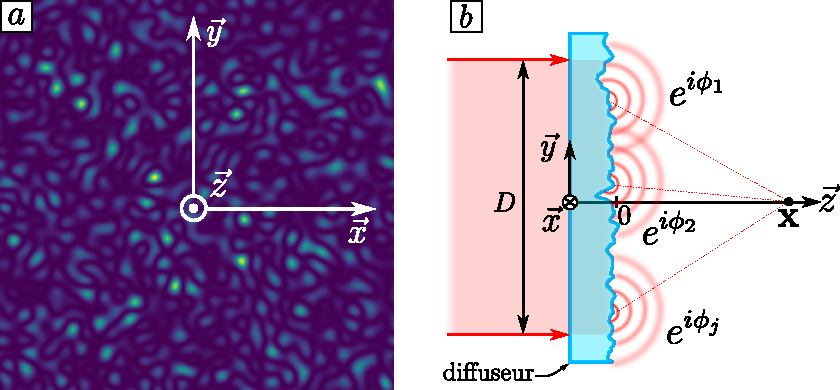
\includegraphics[scale=1]{Fig/Speckle/speckle_pattern.pdf}
\label{fig:speckle_pattern}
\caption{Figure typique de speckle}
\end{figure}

\subsection{Propriétés du diffuseur}

Lame de verre rugueuse, son épaisseur $e(\mathbf{x}_0)$ est une variable aléatoire et donne lieu à une phase $\phi(\mathbf{x}_0)$ elle aussi aléatoire:
\begin{equation}
\phi(\mathbf{x}_0)=2\pi (n-1) \frac{e(\mathbf{x}_0)}{\lambda}
\end{equation}
et donc une transmittance du diffuseur 
\begin{equation}
t_{\mathrm{diff}}(\mathbf{x}_0)=e^{i\phi(\mathbf{x}_0)}
\end{equation}

\begin{equation}
\overline{t_{\mathrm{diff}}} = \overline{e^{i\phi}} = \int{\mathrm{d}\phi \: e^{i\phi} \mathcal{P}(\phi)} \quad\text{avec}\quad \mathcal{P}(\phi)=\frac{1}{\sigma_{\phi} \sqrt{2\pi}} e^{-\frac{(\phi-\overline{\phi})^2}{2\sigma_{\phi}^2}}
\end{equation}
En considérant que $\phi$ est une variable aléatoire gaussienne, ça donne
\begin{equation}
\overline{t_{\mathrm{diff}}}=e^{-\frac{\sigma_{\phi}^2}{2}}
\end{equation}
et en choisissant correctement l'origine temporelle telle que $\overline{\phi}=0$.

On peut aussi écrire $t_{\mathrm{diff}}$ sous la forme
\begin{equation}
t_{\mathrm{diff}}=\overline{t_{\mathrm{diff}}}+\delta t_{\mathrm{diff}}
\end{equation}
ce qui se traduit en terme de champ
\begin{equation}
E=\overline{E}+E_{speckle}
\end{equation}
La conséquence est alors immédiate: si $\sigma_{\phi} \gg 2\pi$ ou de manière équivalente $\sigma_e \gg \lambda$, alors $\overline{t_{\mathrm{diff}}} =0$ et donc le champ rayonné ne sera composé que du champ de speckle: on parle alors de speckle entièrement développé. C'est ce que l'on considèrera dans la suite.

\begin{figure}
\centering
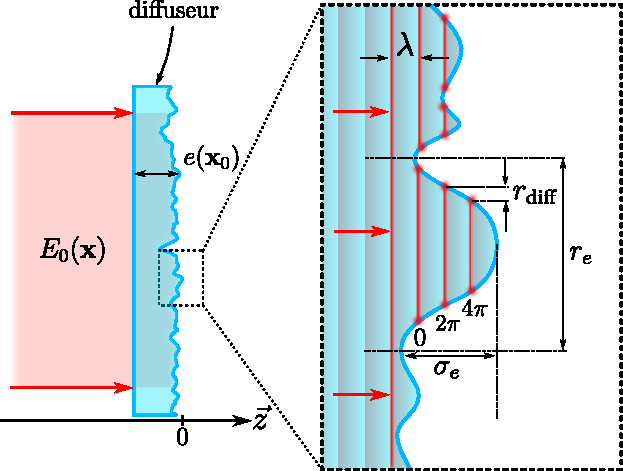
\includegraphics[scale=1]{Fig/Speckle/diffus_prop.pdf}
\label{fig:diffus_prop}
\caption{Caractéristiques du diffuseur. L'épaisseur aléatoire est caractérisée par une hauteur typique $\sigma_e$ et une granularité de taille $r_e$. Pour $\sigma_e \gg \lambda$, on a plusieurs oscillations de l'onde incidente dans le même grain, et donc $t_{\mathrm{diff}}$ qui est une fonction $2\pi-$périodique, voit sa corrélation réduite.}
\end{figure}

Fonction de corrélation: on définit
\begin{equation}
C_{\mathrm{diff}}(\mathbf{x}_0,\mathbf{x}'_0)=\overline{t_{\mathrm{diff}}(\mathbf{x}_0)t^*_{\mathrm{diff}}(\mathbf{x}'_0)}=\overline{e^{i(\phi(\mathbf{x}_0)-\phi(\mathbf{x}'_0))}}
\end{equation}
Si l'on suppose que $\phi(\mathbf{x}_0)-\phi(\mathbf{x}'_0)$ est aussi une variable gaussienne, ça donne
\begin{equation}
C_{\mathrm{diff}}(\mathbf{x}_0,\mathbf{x}'_0)=e^{-\sigma_{\phi}^2 (1-\overline{\phi(\mathbf{x}_0)\phi(\mathbf{x}'_0)}/\sigma_{\phi}^2)}
\end{equation}
Corrélations de l'épaisseur du diffuseur:
\begin{equation}
\frac{\overline{\phi(\mathbf{x}_0)\phi(\mathbf{x}'_0)}}{\sigma_{\phi}^2}=\frac{\overline{e(\mathbf{x}_0)e(\mathbf{x}'_0)}}{\sigma_e^2} \approx 1-\frac{\left| \mathbf{x}_0-\mathbf{x}'_0 \right|^2}{2r_e^2}
\end{equation}
courbe en cloche assez générale valable pour $\left| \mathbf{x}_0 -\mathbf{x}'_0 \right| \ll r_e$.

Au final, ça donne une corrélation de la transmittance 
\begin{equation}
C_{\mathrm{diff}}(\mathbf{x}_0,\mathbf{x}'_0)\approx e^{-\frac{\left| \mathbf{x}_0 - \mathbf{x}'_0 \right| ^2}{2 r_{\mathrm{diff}}^2}}
\end{equation}
avec $r_{\mathrm{diff}} = r_e / \sigma_{\phi}$ la taille effective des grains du diffuseur. Cette taille diminuée s'explique par le fait que si $\sigma_{\phi} \gg 2\pi$, la phase ne sera pas homogène sur la totalité de la largeur d'un grain (de taille typique $r_e$), mais seulement sur une zone réduite. 




\subsection{Statistiques de l'intensité d'un speckle}
Marche aléatoire dans le plan complexe pour $\vec{E}$ car $\sigma_{\phi} \gg 2\pi$ ce qui valide l'approche de marche aléatoire (faire une figure de marche aléatoire avec beaucoup d'angles différents pour monter que $\left\langle t \right\rangle\approx 0$, et que sinon $\left\langle t \right\rangle\neq 0$.

Dans la partie d'avant, c'était au niveau du diffuseur. Maintenant on va s'attacher à décrire ce qu'il se passe après propagation. 
En première approximation, on peut supposer que le champ rayonné est la somme des $N$ champs émis par les diffuseurs avec des phases aléatoires:
\begin{equation}
E(\mathbf{x})=\sum_{j}^{N} E_0 e^{i \phi_j}
\end{equation}
Théorème central limite car $r_{diff} \ll D$, $D$ étant la taille typique de l'éclairement incident.
\begin{equation}
\mathcal{P}(E_{\mathcal{R,I}})=\frac{1}{\sigma_E\sqrt{2\pi}} e^{-\frac{E_{\mathcal{R,I}}^2}{2 \sigma_E^2}}
\end{equation}
avec $E_{\mathcal{R}}$ et $E_{\mathcal{I}}$ les parties réelle et imaginaire du champ complexe $E$ respectivement. En faisant l'intégration angulaire, on trouve 
\begin{equation}
\mathcal{P}(I)=\frac{1}{2\sigma_E^2}e^{-\frac{I}{2\sigma_E^2}}
\end{equation}
Cette loi de probabilité permet alors d'obtenir l'intensité moyenne $\overline{I}=2\sigma_E^2$ et l'écart-type en intensité $\sigma_I=\overline{I}$. Le contraste d'une telle figure de speckle est alors de 1, ce qui se traduit par des pics très brillants entourés de régions sombres d'intensité quasinulle. 


\section{Corrélations spatiales d'un champ de speckle}
\subsection{Implémentation expérimentale}
Présenter brièvement la méthode de mesure des corrélations et surtout la géométrie du problème.

\subsection{Corrélation transverse}
Calcul de la corrélation transverse aux alentours du plan de Fourier, forme gaussienne bien reproduite car la pupille ne coupe que quelques \% de la lumière du faisceau laser gaussien incident: la TF d'une gaussienne faiblement tronquée est une gaussienne correcte.

\subsection{Corrélation longitudinale}
Modélisation en tenant compte des effets non-paraxiaux pour vraiment reproduire la corrélation longitudinale. Calculs lourds numériquement et théoriquement, donc on met en place un modèle paraxial à ON effective.

\section{Propriétés du potentiel de type speckle}
\subsection{Propriétés du potentiel}
Traduction de $P_I(I)$ pour le potentiel dipolaire $V$, Taille des grains de potentiel $\sigma$, potentiel moyen $V_{\mathrm{R}}$, possibilité de faire un potentiel attractif $\delta <0$ ou répulsif $\delta > 0$
\subsection{Possibilité d'un potentiel dépendant de l'état interne}

\section{Potentiel composé d'un speckle bichromatique}
\subsection{S'éloigner de résonance}
Grosse limitation de l'approche précédente utilisée pour les fonctions spectrales: implique qu'on est proche de résonance pour l'état $\left| F=2 \right\rangle$, donc taux d'absorption et d'émission spontanée important: grosse décohérence dans le désordre et donc impossible d'observer la localisation.
Donc on s'éloigne de résonance, donc le potentiel sur $\left| F=1 \right\rangle$ n'est plus négligeable, il faut le compenser: second speckle! 
\subsection{Étude de la similitude de deux speckles}
Physique avec les mains de la similitude entre 2 speckles de longueurs d'onde faiblement différentes. introduction de la finesse $\lambda / \delta\lambda$ ou de la longueur de cohérence $l_{coh}=\lambda^2/\delta\lambda$.
Décorrélation initiale et globale dûe à la propagation dans le diffuseur, puis décorrélation par la différence dans la taille des grains en s'éloignant de l'axe optique.